\chapter{Arhitektura i dizajn sustava}

\noindent Arhitekturu sustava dijelimo na tri različita dijela: \textbf{frontend}, \textbf{backend} i \textbf{bazu podataka}. Jedino koordinirana implementacija ovih podsustava zajedno dovodi do finalnog proizvoda u obliku web platforme koju ostvarujemo. 
\newline \newline
\noindent \textbf{\textit{Frontend}} predstavlja sučelje između korisnika i same platforme. Konkretno, on pruža korisniku pregled sadržaja web stranice i omogućava mu komunikaciju s aplikacijom putem \textit{HTTP} (\textit{HyperText Transfer Protocol}) zahtjeva.
\newline\newline\noindent \textbf{\textit{Backend}} je taj koji te zahtjeve obrađuje i upravlja podatcima u bazi podataka. Neke od funkcionalnosti koje omogućuje backend su primjerice registracija novog korisnika ili brisanje korisnika od strane sistemskog administratora. 
\newline\newline\noindent \textbf{\textit{Baza podataka}} spremište je entiteta koji su prikazani u obliku tablica s atributima. Iz nje se često čitaju podatci i po potrebi ažuriraju. Kritičan je dio arhitekture sustava. 
 \textbf{\newline\newline\noindent Controller - Service - Repository} troslojna arhitektura temelj je backend implementacije aplikacije. \textit{Controller} sloj povezuje frontend i backend, pozivajući \textit{Service} sloj da obradi zahtjeve korisnika. Ako je za obradu tih zahtjeva potreban pristup bazi podataka, Service sloj poziva funkcije \textit{Repository} sloja koji to omogućuje. 
 \newline\newline\noindent Frontend je implementiran uz pomoć \textit{JavaScripta} (radnog okvira \textit{React.js}), \textit{HTML-a} i \textit{CSS-}a. Za backend je korišten programski jezik \textit{Java} (radni okvir \textit{Spring Boot}), a odabrana je razvojna okolina \textit{Intellij IDEA}. Ispitivanje backend funkcionalnosti omogućeno je korištenjem \textit{Postman} platforme. Baza podataka izgrađena je korištenjem \textit{PostgreSQL} sustava za upravljanje bazom podataka. Aplikacija je stavljena u pogon na \textit{Render} servisu. 

		\section{Baza podataka}
			
		Za našu platformu koristit ćemo relacijsku bazu podataka. Objekt takve baze je relacija, odnosno tablica koja je definirana svojim imenom i skupom atributa. Atributi unutar jednog entiteta mogu poprimiti funkciju primarnog ili stranog ključa.
Baza podataka u našem se slučaju sastoji se od 2 entiteta - \textbf{profile} i \textbf{recipe}.
		
			\subsection{Opis tablica}

\noindent \textbf{\textit{profile}}\\
\begin{samepage}
Ovaj entitet sadrži osnovne informacije o korisničkom profilu i  sastoji se od sljedećih atributa: \textit{userID} (autogenerirani identifikator korisnika), \textit{email }(e-mail adresa), \textit{username} (korisničko ime), \textit{password} (lozinka), \textit{name} (ime), \textit{surname} (prezime) i \textit{age} (dob). Atribut\textit{ userID} primarni je ključ entiteta \textbf{profile}. 
\end{samepage}

    				\begin{longtblr}[
					label=none,
					entry=none
					]{
						width = \textwidth,
						colspec={|X[6,l]|X[6, l]|X[20, l]|}, 
						rowhead = 1,
					} %definicija širine tablice, širine stupaca, poravnanje i broja redaka naslova tablice
     
					\hline \SetCell[c=3]{c}{\textbf{profile}}	 \\ \hline[3pt]
					\SetCell{LightGreen}userID & VARCHAR	&  	jedinstveni identifikator korisnika	\\ \hline
					\SetCell{}email & VARCHAR	&  	jedinstvena e-mail adresa korisnika 	\\ \hline
     				\SetCell{}username & VARCHAR	&  	jedinstveno korisničko ime	\\ \hline
					\SetCell{} password & VARCHAR	&  lozinka korisnika 	\\ \hline
          			\SetCell{} name & VARCHAR	&  ime korisnika (opcionalno)	\\ \hline
               		\SetCell{} surname & VARCHAR	&  	prezime korisnika (opcionalno)	\\ \hline
                    \SetCell{} age & INT	&  	dob korisnika (opcionalno)	\\ \hline
                    
				\end{longtblr}

    
\noindent \textbf{\textit{recipe}}\\
\begin{samepage}
Ovaj entitet opisuje recept postavljen na platformu od strane registriranog korisnika. Primarni je ključ entiteta \textit{recipeID} (autogenerirani identifikator recepta), a strani ključ \textit{userID} koji povezuje entitete \textbf{recipe} i \textbf{profile}.
\end{samepage}
\eject

\begin{samepage}
\noindent Ostali atributi su: \textit{likes} (broj oznaka "sviđa mi se" na receptu od strane registriranih korisnika), koji je inicijalno postavljen na 0, \textit{ingredients} (sastojci jela koje recept opisuje), \textit{name} (ime recepta), \textit{instructions} (niz uputa pripreme jela opisanog receptom), \textit{origin} (mjesto podrijetla jela), \textit{category} (kategorija jela), \textit{specialTags} (dodatne oznake), \textit{imageURL} (URL slike koju korisnik prilaže uz postavljeni recept), \textit{videoURL} (URL videa koji korisnik prilaže uz postavljeni recept) te \textit{preparationTime} (vrijeme potrebno za spremanje receptnog jela).
\end{samepage}
    
    				\begin{longtblr}[
					label=none,
					entry=none
					]{
						width = \textwidth,
						colspec={|X[8, l]|X[6, l]|X[20, l]|}, 
						rowhead = 1,
					} %definicija širine tablice, širine stupaca, poravnanje i broja redaka naslova tablice
					\hline \SetCell[c=3]{c}{\textbf{recipe}}	 \\ \hline[3pt]
					\SetCell{LightGreen}recipeID & VARCHAR	&  	jedinstveni identifikator recepta 	\\ \hline
               		\SetCell{} likes & INT	&  	broj oznaka "sviđa mi se" recepta 	\\ \hline
                    \SetCell{} ingredients & VARCHAR	&  	popis sastojaka receptnog jela 	\\ \hline
                    \SetCell{} name & VARCHAR	&  	ime recepta 	\\ \hline
                    \SetCell{} instructions & VARCHAR	&  	niz uputa za pripremu jela prema receptu 	\\ \hline
                    \SetCell{} origin & VARCHAR	&  	mjesto podrijetla receptnog jela (opcionalno)	\\ \hline
                    \SetCell{} category & VARCHAR	&  	vrsta (kategorija) receptnog jela	\\ \hline
                    \SetCell{} specialTags & VARCHAR	&  	specijalne dodatne oznake receptnog jela (opcionalno)	\\ \hline
                    \SetCell{} imageURL & VARCHAR	&  	URL slike priložene uz recept 	\\ \hline
					\SetCell{} videoURL & VARCHAR	&  	URL videa priloženog uz recept (opcionalno)	\\ \hline
    				\SetCell{} preparationTime & INT	&  	vrijeme kuhanja jela u minutama	\\ \hline
					\SetCell{LightBlue}userID & VARCHAR	&  	jedinstveni identifikator korisnika 	\\ \hline
				\end{longtblr}
				
				
			
			\subsection{Dijagram baze podataka}
			
			\begin{figure}[H]
			    \centering
			    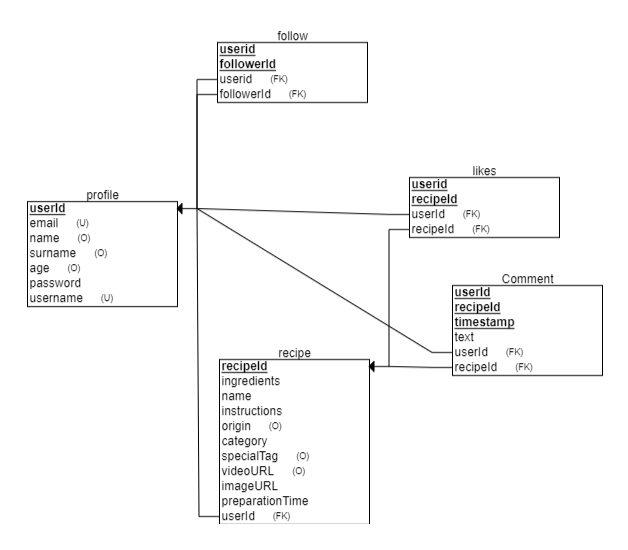
\includegraphics[width=1\linewidth]{slike/DBdiagram.png}
			    \caption{Dijagram baze podataka}
			    \label{fig:enter-label}
			\end{figure}
			
			\eject
			
			
		\section{Dijagram razreda}
			
			\textbf{\textit{dio 1. revizije}}\\
			
			\textit{Prilikom prve predaje projekta, potrebno je priložiti potpuno razrađen dijagram razreda vezan uz \textbf{generičku funkcionalnost} sustava. Ostale funkcionalnosti trebaju biti idejno razrađene u dijagramu sa sljedećim komponentama: nazivi razreda, nazivi metoda i vrste pristupa metodama (npr. javni, zaštićeni), nazivi atributa razreda, veze i odnosi između razreda.}\\

\begin{figure}[H]
			    \centering
			    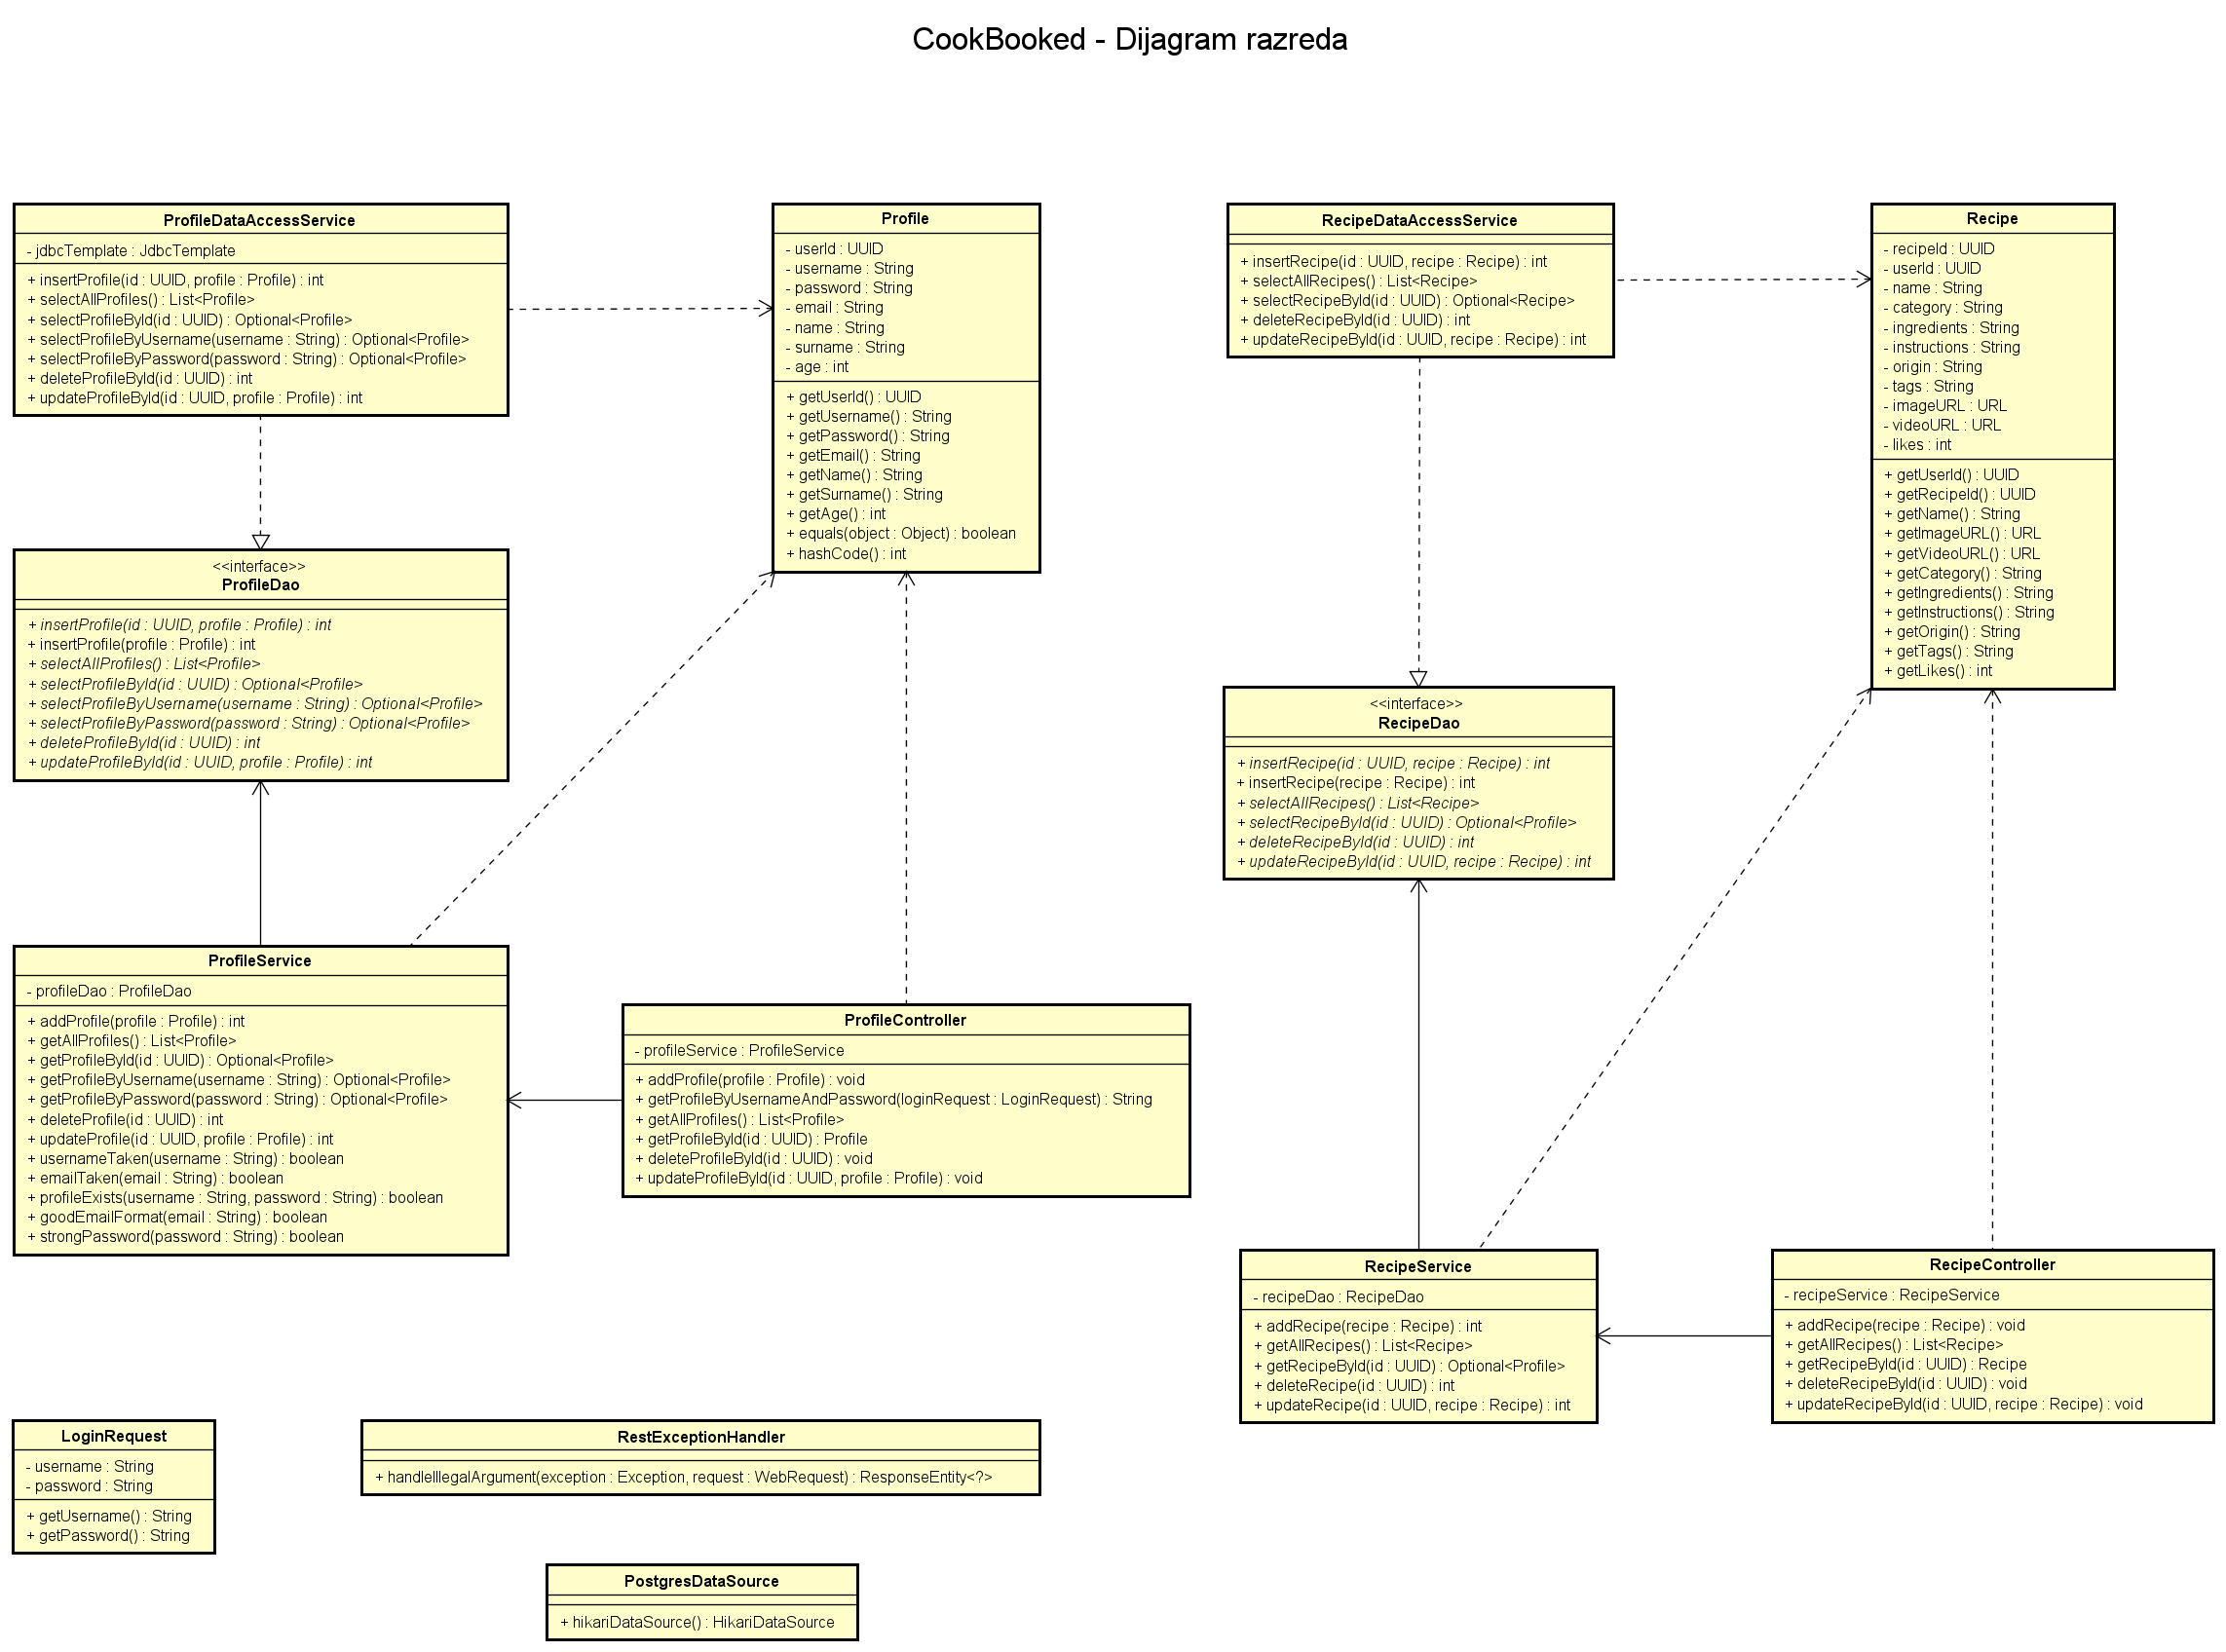
\includegraphics[width=1\linewidth]{slike//dijagrami/Dijagram razreda.png}
			    \caption{Dijagram razreda}
			    \label{fig:enter-label}
			\end{figure}
	\eject		
   \textbf{\textit{dio 2. revizije}}\\			
			
			\textit{Prilikom druge predaje projekta dijagram razreda i opisi moraju odgovarati stvarnom stanju implementacije}
			
			
			
			\eject
		
		\section{Dijagram stanja}
			
			
			\textbf{\textit{dio 2. revizije}}\\
			
			\textit{Potrebno je priložiti dijagram stanja i opisati ga. Dovoljan je jedan dijagram stanja koji prikazuje \textbf{značajan dio funkcionalnosti} sustava. Na primjer, stanja korisničkog sučelja i tijek korištenja neke ključne funkcionalnosti jesu značajan dio sustava, a registracija i prijava nisu. }
			
			
			\eject 
		
		\section{Dijagram aktivnosti}
			
			\textbf{\textit{dio 2. revizije}}\\
			
			 \textit{Potrebno je priložiti dijagram aktivnosti s pripadajućim opisom. Dijagram aktivnosti treba prikazivati značajan dio sustava.}
			
			\eject
		\section{Dijagram komponenti}
		
			\textbf{\textit{dio 2. revizije}}\\
		
			 \textit{Potrebno je priložiti dijagram komponenti s pripadajućim opisom. Dijagram komponenti treba prikazivati strukturu cijele aplikacije.}
